\documentclass[11pt,a4paper,oneside]{report}             % Single-side
%\documentclass[11pt,a4paper,twoside,openright]{report}  % Duplex

\usepackage{ifxetex}
\ifxetex
  \usepackage{fontspec}
\else
  \usepackage[T1]{fontenc}
  \usepackage[utf8]{inputenc}
  \usepackage{lmodern}
\fi

\usepackage[english,magyar]{babel} % Alapértelmezés szerint utoljára definiált nyelv lesz aktív, de később külön beállítjuk az aktív nyelvet.

\usepackage{cmap}
\usepackage{amsfonts,amsmath,amssymb} % Mathematical symbols.
\usepackage[ruled,boxed,resetcount,linesnumbered]{algorithm2e} % For pseudocodes.
\usepackage{booktabs} % For publication quality tables for LaTeX
\usepackage{graphicx}

%\usepackage{fancyhdr}
%\usepackage{lastpage}

\usepackage{anysize}
\usepackage{sectsty}
\usepackage{setspace}  % Ettol a tablazatok, abrak, labjegyzetek maradnak 1-es sorkozzel!

\usepackage{hyperref} % For hyperlinks in the generated document. 
\usepackage{color}
\usepackage{listings} % For source code snippets.

\usepackage[amsmath,thmmarks]{ntheorem} % Theorem-like environments.

\usepackage[hang]{caption}



%--------------------------------------------------------------------------------------
% Language configuration
%--------------------------------------------------------------------------------------
%--------------------------------------------------------------------------------------
% Elnevezések
%--------------------------------------------------------------------------------------
\newcommand{\dolgozatnyelve}{\selectlanguage{english}}

\newcommand{\bme}{Budapest University of Technology and Economics}
\newcommand{\vik}{Faculty of Electrical Engineering and Informatics}

\newcommand{\bmemit}{Department of Measurement and Information Systems}

\newcommand{\keszitette}{Author}
\newcommand{\konzulens}{Advisor}

\newcommand{\bsc}{Bachelor's Thesis}
\newcommand{\msc}{Master's Thesis}

\newcommand{\pelda}{Example}
\newcommand{\definicio}{Definition}
\newcommand{\tetel}{Theorem}

\newcommand{\bevezeto}{Introduction}
\newcommand{\koszonetnyilvanitas}{Acknowledgements}
\newcommand{\abrakjegyzeke}{List of Figures}
\newcommand{\tablazatokjegyzeke}{List of Tables}
\newcommand{\kodreszletekjegyzeke}{List of Code Listings}
\newcommand{\irodalomjegyzek}{Bibliography}
\newcommand{\fuggelek}{Appendix}


\newcommand{\englishParagraph}{
	\setlength{\parindent}{0em} % angol nyelvű dokumentumokban jellemző
	\setlength{\parskip}{0.5em} % angol nyelvű dokumentumokban jellemző
	\nonfrenchspacing
}

\newcommand{\hungarianParagraph}{
	\setlength{\parindent}{2em} % angol nyelvű dokumentumokban jellemző
	\setlength{\parskip}{0em}   % angol nyelvű dokumentumokban jellemző
	\frenchspacing
}

\newcommand{\defaultParagraph}{
	\englishParagraph
} % Settings for English documents


%--------------------------------------------------------------------------------------
% Main variables
%--------------------------------------------------------------------------------------
\newcommand{\vikszerzo}{Unicsovics Milán György} % Szerző neve
\newcommand{\vikkonzulensA}{Dr. Micskei Zoltán} % Első konzulens neve
\newcommand{\vikkonzulensB}{} % Második konzulens neve; hagyd üresen, ha egy konzulensed van.
\newcommand{\vikcim}{Test generation based on state machine models} % Cím
\newcommand{\viktanszek}{\bmemit} % Tanszék
\newcommand{\vikdoktipus}{\msc} % Dokumentum típusa

%--------------------------------------------------------------------------------------
% Page layout setup
%--------------------------------------------------------------------------------------
% we need to redefine the pagestyle plain
% another possibility is to use the body of this command without \fancypagestyle
% and use \pagestyle{fancy} but in that case the special pages
% (like the ToC, the References, and the Chapter pages)remain in plane style

\pagestyle{plain}
\marginsize{35mm}{25mm}{15mm}{15mm}

\setcounter{secnumdepth}{0}
\sectionfont{\large\upshape\bfseries}
\setcounter{secnumdepth}{2}

\sloppy % Margón túllógó sorok tiltása.
\widowpenalty=10000 \clubpenalty=10000 %A fattyú- és árvasorok elkerülése
\def\hyph{-\penalty0\hskip0pt\relax} % Kötőjeles szavak elválasztásának engedélyezése


%--------------------------------------------------------------------------------------
% Setup hyperref package
%--------------------------------------------------------------------------------------
\hypersetup{
    bookmarks=true,            % show bookmarks bar?
    unicode=false,              % non-Latin characters in Acrobat's bookmarks
    pdftitle={\vikcim},        % title
    pdfauthor={\vikszerzo},    % author
    pdfsubject={\vikdoktipus}, % subject of the document
    pdfcreator={\vikszerzo},   % creator of the document
    pdfproducer={},    % producer of the document
    pdfkeywords={MBT, Java, Acceleo, Alloy},
                                  % list of keywords (separate then by comma)
    pdfnewwindow=true,         % links in new window
    colorlinks=true,           % false: boxed links; true: colored links
    linkcolor=black,           % color of internal links
    citecolor=black,           % color of links to bibliography
    filecolor=black,           % color of file links
    urlcolor=black             % color of external links
}


%--------------------------------------------------------------------------------------
% Set up listings
%--------------------------------------------------------------------------------------
\definecolor{lightgray}{rgb}{0.95,0.95,0.95}
\lstset{
	basicstyle=\scriptsize\ttfamily, % print whole listing small
	keywordstyle=\color{black}\bfseries, % bold black keywords
	identifierstyle=, % nothing happens
	commentstyle=\color{green}, % green comments
	stringstyle=\scriptsize,
	showstringspaces=false, % no special string spaces
	aboveskip=3pt,
	belowskip=3pt,
	backgroundcolor=\color{lightgray},
	columns=flexible,
	numbers=left,
    numberstyle=\tiny\color{black},
    numbersep=10pt,
	keepspaces=true,
	escapeinside={(*@}{@*)},
	literate=*
		{á}{{\'a}}1	{é}{{\'e}}1	{í}{{\'i}}1	{ó}{{\'o}}1	{ö}{{\"o}}1	{ő}{{\H{o}}}1	{ú}{{\'u}}1	{ü}{{\"u}}1	{ű}{{\H{u}}}1
		{Á}{{\'A}}1	{É}{{\'E}}1	{Í}{{\'I}}1	{Ó}{{\'O}}1	{Ö}{{\"O}}1	{Ő}{{\H{O}}}1	{Ú}{{\'U}}1	{Ü}{{\"U}}1	{Ű}{{\H{U}}}1
}
\def\lstlistingname{Listing}


%--------------------------------------------------------------------------------------
% Set up theorem-like environments
%--------------------------------------------------------------------------------------
% Using ntheorem package -- see http://www.math.washington.edu/tex-archive/macros/latex/contrib/ntheorem/ntheorem.pdf

\theoremstyle{plain}
\theoremseparator{.}
\newtheorem{example}{\pelda}

\theoremseparator{.}
%\theoremprework{\bigskip\hrule\medskip}
%\theorempostwork{\hrule\bigskip}
\theorembodyfont{\upshape}
\theoremsymbol{{\large \ensuremath{\centerdot}}}
\newtheorem{definition}{\definicio}

\theoremseparator{.}
%\theoremprework{\bigskip\hrule\medskip}
%\theorempostwork{\hrule\bigskip}
\newtheorem{theorem}{\tetel}


%--------------------------------------------------------------------------------------
% Some new commands and declarations
%--------------------------------------------------------------------------------------
\newcommand{\code}[1]{{\upshape\ttfamily\scriptsize\indent #1}}
\newcommand{\doi}[1]{DOI: \href{http://dx.doi.org/\detokenize{#1}}{\raggedright{\texttt{\detokenize{#1}}}}} % A hivatkozások közt így könnyebb DOI-t megadni.

\DeclareMathOperator*{\argmax}{arg\,max}
%\DeclareMathOperator*[1]{\floor}{arg\,max}
\DeclareMathOperator{\sign}{sgn}
\DeclareMathOperator{\rot}{rot}


%--------------------------------------------------------------------------------------
% Setup captions
%--------------------------------------------------------------------------------------
\captionsetup[figure]{
	width=.75\textwidth,
	aboveskip=10pt}

\renewcommand{\captionlabelfont}{\bf}
%\renewcommand{\captionfont}{\footnotesize\it}


%--------------------------------------------------------------------------------------
% Redefine reference style
%--------------------------------------------------------------------------------------
\newcommand{\figref}[1]{\ref{fig:#1}.}
\renewcommand{\eqref}[1]{(\ref{eq:#1})}
\newcommand{\listref}[1]{\ref{listing:#1}.}
\newcommand{\sectref}[1]{\ref{sect:#1}}
\newcommand{\tabref}[1]{\ref{tab:#1}.}


%--------------------------------------------------------------------------------------
% Hyphenation exceptions
%--------------------------------------------------------------------------------------
\hyphenation{Shakes-peare Mar-seilles ár-víz-tű-rő tü-kör-fú-ró-gép}


\author{\vikszerzo}
\title{\viktitle}

\renewcommand*{\lstlistlistingname}{List of Code Listings}


%--------------------------------------------------------------------------------------
% Table of contents and the main text
%--------------------------------------------------------------------------------------
\begin{document}


%~~~~~~~~~~~~~~~~~~~~~~~~~~~~~~~~~~~~~~~~~~~~~~~~~~~~~~~~~~~~~~~~~~~~~~~~~~~~~~~~~~~~~~
	\selectlanguage{english}
	%--------------------------------------------------------------------------------------
%	The title page
%--------------------------------------------------------------------------------------
\begin{titlepage}
\begin{center}

\includegraphics[width=60mm,keepaspectratio]{figures/bme_logo.pdf}\\
\vspace{0.3cm}
\textbf{\bme}\\
\textmd{\vik}\\
\textmd{\viktanszek}\\[5cm]

\vspace{0.4cm}
{\huge \bfseries \vikcim}\\[0.8cm]
\vspace{0.5cm}
\textsc{\Large \vikdoktipus}\\[4cm]

{
	\renewcommand{\arraystretch}{0.85}
	\begin{tabular}{cc}
	 \makebox[7cm]{\emph{\keszitette}} & \makebox[7cm]{\emph{\konzulens}} \\ \noalign{\smallskip}
	 \makebox[7cm]{\vikszerzo} & \makebox[7cm]{\vikkonzulensA} \\
	  & \makebox[7cm]{\vikkonzulensB} \\
	\end{tabular}
}

\vfill
{\large \today}
\end{center}
\end{titlepage}


		% Diploma

% Table of Contents
%~~~~~~~~~~~~~~~~~~~~~~~~~~~~~~~~~~~~~~~~~~~~~~~~~~~~~~~~~~~~~~~~~~~~~~~~~~~~~~~~~~~~~~
	\pagenumbering{gobble}
	\onehalfspacing
	\tableofcontents\newpage


% Declaration and Abstract
%~~~~~~~~~~~~~~~~~~~~~~~~~~~~~~~~~~~~~~~~~~~~~~~~~~~~~~~~~~~~~~~~~~~~~~~~~~~~~~~~~~~~~~
	% Hallgatói nyilatkozat
	\selectlanguage{magyar}
\pagenumbering{gobble}
%--------------------------------------------------------------------------------------
% Nyilatkozat
%--------------------------------------------------------------------------------------
\begin{center}
\large
\textbf{HALLGATÓI NYILATKOZAT}\\
\end{center}

Alulírott \emph{\vikszerzo}, szigorló hallgató kijelentem, hogy ezt a  diplomatervet meg nem engedett segítség nélkül, saját magam készítettem, csak a megadott forrásokat (szakirodalom, eszközök stb.) használtam fel. Minden olyan részt, melyet szó szerint, vagy azonos értelemben, de átfogalmazva más forrásból átvettem, egyértelműen, a forrás megadásával megjelöltem.

Hozzájárulok, hogy a jelen munkám alapadatait (szerző(k), cím, angol és magyar nyelvű tartalmi kivonat, készítés éve, konzulens(ek) neve) a BME VIK nyilvánosan hozzáférhető elektronikus formában, a munka teljes szövegét pedig az egyetem belső hálózatán keresztül (vagy autentikált felhasználók számára) közzétegye. Kijelentem, hogy a benyújtott munka és annak elektronikus verziója megegyezik. Dékáni engedéllyel titkosított diplomatervek esetén a dolgozat szövege csak 3 év eltelte után válik hozzáférhetővé.

\begin{flushleft}
\vspace*{1cm}
Budapest, \today
\end{flushleft}

\begin{flushright}
 \vspace*{1cm}
 \makebox[7cm]{\rule{6cm}{.4pt}}\\
 \makebox[7cm]{\emph{\vikszerzo}}\\
 \makebox[7cm]{hallgató}
\end{flushright}
\thispagestyle{empty}

\vfill
\clearpage
\thispagestyle{empty} % an empty page

\dolgozatnyelve

	%TODO Összefoglaló
	\pagenumbering{roman}
\setcounter{page}{1}

\selectlanguage{magyar}
\hungarianParagraph


%----------------------------------------------------------------------------
% Abstract in Hungarian
%----------------------------------------------------------------------------
\chapter*{Kivonat}\addcontentsline{toc}{chapter}{Kivonat}

Jelen dokumentum egy diplomaterv sablon, amely formai keretet ad a BME Villamosmérnöki és Informatikai Karán végző hallgatók által elkészítendő szakdolgozatnak és diplomatervnek. A sablon használata opcionális. Ez a sablon \LaTeX~alapú, a \emph{TeXLive} \TeX-implementációval és a PDF-\LaTeX~fordítóval működőképes.


\vfill
\selectlanguage{english}
\englishParagraph


%----------------------------------------------------------------------------
% Abstract in English
%----------------------------------------------------------------------------
\chapter*{Abstract}\addcontentsline{toc}{chapter}{Abstract}

This document is a \LaTeX-based skeleton for BSc/MSc~theses of students at the Electrical Engineering and Informatics Faculty, Budapest University of Technology and Economics. The usage of this skeleton is optional. It has been tested with the \emph{TeXLive} \TeX~implementation, and it requires the PDF-\LaTeX~compiler.


\vfill
\dolgozatnyelve
\defaultParagraph

\newcounter{romanPage}
\setcounter{romanPage}{\value{page}}
\stepcounter{romanPage}

	\clearpage\pagenumbering{arabic}


% The main part of the thesis
%~~~~~~~~~~~~~~~~~~~~~~~~~~~~~~~~~~~~~~~~~~~~~~~~~~~~~~~~~~~~~~~~~~~~~~~~~~~~~~~~~~~~~~

	%TODO Bevezetés
	%----------------------------------------------------------------------------
\chapter{Introduction}
\label{cha:introduction}
%----------------------------------------------------------------------------

\section{Problem and thesis statement}
\label{sec:problem}

...

% section problem (end)

\section{Proposed approach}
\label{sec:proposedapproach}

...

% section proposedapproach (end)

% chapter introduction (end)
	%TODO Modell alapú tesztelés
	%----------------------------------------------------------------------------
\chapter{Model-based testing}
\label{cha:modelbasedtesting}
%----------------------------------------------------------------------------

The idea of model-based testing originates from the 70's and now it has an extensive literature, terminology and a commonly accepted taxonomy \cite{taxonomy}. MBT can be defined as a software testing technique, where the software's intended behaviour is verified against a formerly constructed model. This chapter introduces the concept of this variant of software testing through a concrete process (Figure~\ref{fig:mbtprocess}).

\begin{figure}[htp]
\centering
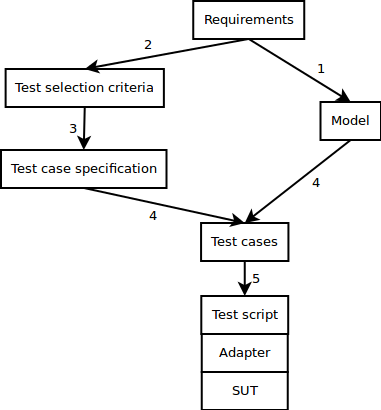
\includegraphics[scale=0.55]{figures/mbt_process.png}
\caption{Model-based testing process}
\label{fig:mbtprocess}
\end{figure}

\begin{description}
    \item[1. Modelling] From informal requirements or previously defined specifications a model can be built. The model is an abstract representation of the \textit{system under test (SUT)}. It uses encapsulation for information reduction, because it has to be more simple, than the original system to achieve an easier modifying and maintaining \cite{mbttestcasegeneration}. During model-based software development the model can be used for many other tasks too, as it serves analysing, synthesising and documenting the SUT as well.
     \item[2. Test planning] \textit{Test selection criteria} decide how the test cases are chosen, which point of view is important by testing. Later these selected criteria will control the whole test generation process. Criteria are transformed into \textit{test case specifications}, which are the formalised versions of the criteria. These two steps are often treated separately, but they form a cohesive step of test planning, thus they will be discussed together in this thesis.
     \item[3. Test generation] After creating the model and the test case specifications set of \textit{test cases} is generated automatically from the model regarding all the specifications. One of the biggest challenges is to create the test cases. A simple test case consists of a pair of input parameters and expected outputs. Finite set of test cases forms a \textit{test suite}. The difficulty comes from the need to satisfy the test case specifications and create a minimised set of test cases.
     \item[4. Test execution] A successfully generated test suite can be executed on the SUT. For the execution a \textit{test script} can be used, which executes the test cases.
     
     The generated test cases are strongly linked to the abstract test model, therefore an \textit{adaptor} component is needed, which is often part of the test script. The adaptor adapts the test inputs to the SUT. For example if the input of a method is an XML document containing an integer value, the adaptor has to transform the test case's test inputs to XML.
     
     The test script also contains usually a \textit{test oracle}, that checks the test output difference from the expected output.
\end{description}

Utting, Pretschner and Legeard investigated the currently available MBT solutions and defined a taxonomy (see Figure~\ref{fig:mbttaxonomy}) which concentrates to three major properties of model-based testing. The three dimensions of their taxonomy are the modelling specification, test generation and test execution, which will be followed and expanded by the presentation of each stages of the testing process.

\section{Modelling}
\label{sec:modelling}

The first step of the model based testing process is to create a suitable model, from which a test suite can be generated.  Model specifications has three dimension considering the different MBT approaches.

\begin{description}
	\item[Model scope] The scope of the modelling is a binary decision. The model either specify \textit{just the test input} or \textit{the input-output pairs} for the SUT. Usually the first case is less useful, because the test script can not check the SUT's output and that's why it is difficult to create an oracle that way.
	
	\item[Model characteristics] The SUT assigns the main characteristics of the model. It depends on the SUT's timing properties (\textit{timed} / \textit{untimed}), determinism (\textit{deterministic} / \textit{non-deterministic}) and dynamics (\textit{discrete} / \textit{continuous} / \textit{hybrid}).
	
	\item[Model paradigm] The third dimension is the paradigm that is used to describe the model. \textit{State-based notation} means, that set of variables defines the model, which represents the internal state of the system and there are some operations that modify those variables. Usually these operations given by preconditions and postconditions. By \textit{transition-based notation} the model focuses on the transition between the state of the system. Finite state machines are examples of this paradigm. \textit{History-based notations} model the allowable traces of its behaviour over time. By \textit{functional notation} collection of mathematical functions model the system. \textit{Operational notations} describe the model as a set of executable processes running parallel. Petri nets are good forms of this notation. \textit{Stochastic notations} describe the model by a probabilistic model, so it is rather suitable to model the environment than the SUT itself. An example can be the Markov chains for this type of model paradigm. The last paradigm is the \textit{data-flow notation}, where the main concept is the concentration to the data, rather than the control flow, example can be the often used Matlab Simulink model.
\end{description}

\begin{figure}[htp]
\centering
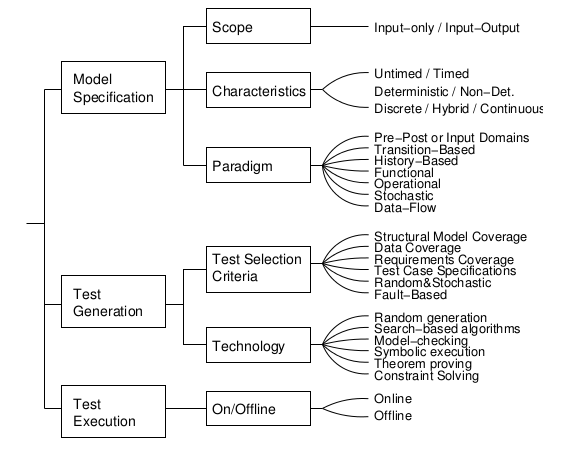
\includegraphics[scale=0.5]{figures/mbt_taxonomy.png}
\caption{Model-based testing taxonomy \cite{taxonomy}}
\label{fig:mbttaxonomy}
\end{figure}

As we saw by the taxonomy, all the identified model paradigms used in model-based testing belong to some kind of behaviour modelling notation. This is not a surprise, because a data or functional model can not be utilised so effectively by software testing. Each model paradigm concentrates to a different aspect of the behaviour.

There is a plethora of technologies for modelling behaviour and one of the most frequently used are the extended finite state machine (EFSM) and all of its variations. These variations mostly use transition based notation, but they can combine it with other modelling paradigms as well. The second most popular modelling language according to Shafique and Labiche \cite{toolsreview} is the UML state machine language, which is an enhanced version of EFSMs. Other modelling languages are used in the field of MBT too, but mostly these tools made for a specific purpose.

As EFSMs or at least their variations serve as basic modelling notation for the most available model based testing tools, that's why we have to investigate them properly. The basic parts of the UML language will be described here as well.

\subsection{Extended finite state machines}
\label{sub:efsm}

A \textit{finite state machine} is a 6-tuple $\langle S, I, A, R, \Delta, T\rangle$, where
\begin{align*}
& S: \text{set of finite states},\\
& I \subset S: \text{set of initial states},\\
& A: \text{finite alphabet of input symbols},\\
& R: \text{set of possible outputs},\\
& \Delta \subset S \times A: \text{set of possible input relations},\\
& T: \text{is a transition relation function}\ f: \Delta \rightarrow S \times R
\end{align*}

The semantic of this model is the following. When $T(s, a) = (s', r)$, the state machine is receiving an input $a \in A$ in state $s \in S$, assuming $(s,a) \in \Delta$, then the system moves to the new state $s' \in S$ and outputs $r \in R$. A possible $(s'', a') \notin \Delta$ is interpreted as an input symbol that is not allowed in that state.

An \textit{extended finite state machine} differs from a simple finite state machine in terms of the states defined differently. The states of an extended state machine has the form $S = D_0 \times D_1 \times \dots D_n$, where $D_0$ is the set of control states, and $D_{i=1}^n$ is the domain of state variables $x_i$, that are assigned to each states.

% subsection efsm (end)

\subsection{UML state machines}
\label{sub:umlstatemachine}

UML state machines or UML state charts are improved versions of the mathematical concept of finite state machines expressed with the OMG's Unified Modeling Language \cite{omguml}. The original FSM notations suffers greatly by the state and transition explosion problem, because the complexity of these models tend to grow faster as the modelled system. UML state machines solved this problem by extracting the common parts of these system and sharing the common behaviour across the states.

The idea behind the notation is that an entity or each of its sub-entities is always in exactly one of the possible states and there are well-defined conditional transitions between these states. There are two kinds of state machine, which can be used to define behaviour of model elements or to describe protocol usage.

\begin{figure}[htp]
\centering
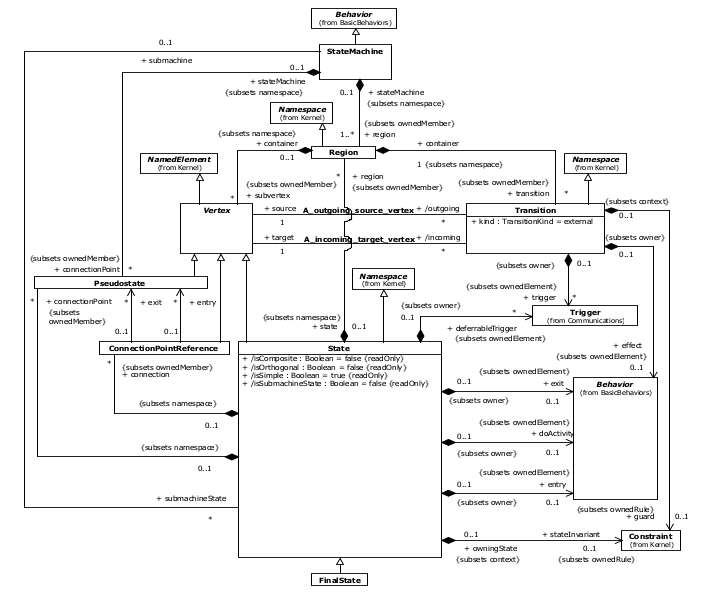
\includegraphics[scale=0.6]{figures/statemachine_metamodel}
\caption{Metamodel of UML state machine \cite{omguml}}
\label{fig:statemachine_metamodel}
\end{figure}

UML state machines are similar to FSMs, but they also have differences. For example UML state charts introduce new features over traditional finite machines such as hierarchically nested regions, orthogonal regions, entry/exit actions, internal transitions and transition execution sequences. The main concepts of this notation are discussed separately.

\begin{description}
	\item[States] are the phases of the system's history. For example if the history can be separated into two phases, then there are two states. 
	\item[Extended states] represents the complete condition of the system. This interpretation means usually states extended with system variables.
	\item[Transitions] happens when a state switched to another.
	\item[Actions] executed when an event dispatched and the system responds by performing them.
	\item[Events] can be everything, that affects the system, and causes state change.
	
\begin{figure}[htp]
\centering
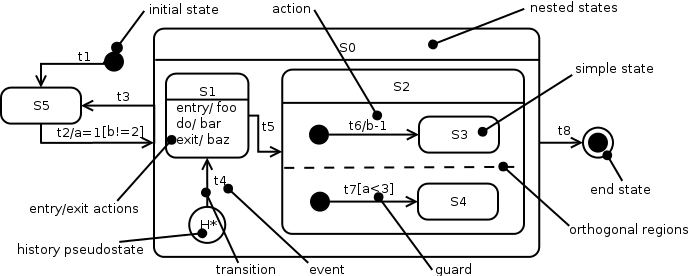
\includegraphics[scale=0.5]{figures/mbt_smexample}
\caption{Example UML state machine}
\label{fig:mbt_smexample}
\end{figure}
	
	\item[Guards] are boolean expressions described with extended state variables and event parameters. They can affect the system's behaviour by enabling or disabling transitions.
	\item[Hierarchically nested regions] means that if a system is in a substate then it is also in the same time in all the substate's superstates.
	\item[Orthogonal regions] are regions, which are either in 'OR'  or 'AND' relation.
	\item[Entry/exit actions] are actions which are dispatched upon entry to a state or exit from it.
	\item[Internal transitions] do not cause state transitions, but only some internal actions to execute and the actual state stays the same.
	\item[Transition execution sequence] describes an execution sequence of actions to do upon event dispatching. First the guard of the transition evaluates. Then the exit actions of the source state configuration will be executed. Then come the actions associated with the transition. Finally the entry actions of the target state configuration will be executed.
\end{description}

% subsection umlstatemachine (end)

% section modelling (end)

\section{Test planning}
\label{sec:testplanning}

Planning tests involves two steps considering the model based test generation process. At first the test selection criteria are chosen, which will be formalised into a test case specification later on.

Test selection criteria control the test case generation. MBT taxonomy includes the following identified criteria. \textit{Structural model coverage criteria} aim to cover a part of the model, for example nodes and arcs of the transition-based model. The nodes of such a model represent the states of the system, and the arcs represent the transitions respectively. The basic idea of \textit{data coverage criteria} is to split the data space to equivalence classes and choose values from them. \textit{Requirements based coverage criteria} are linked to the informal requirements of the SUT and it applies the coverage to the requirements. \textit{Ad-hoc test case specifications} guides by the test case specifications. \textit{Random and stochastic criteria} are useful rather to model the environment and applicable to use with a stochastic model. \textit{Fault-based criteria} can be very efficient, because it concentrates to error finding in the SUT.

The main goal of the test selection criteria is to guide the automatic test selection by the test case generation. A good criteria fulfils the previously defined testing policy and testing strategy, that were specified for the system \cite{istqb}. Testing policies give rules for testing, while strategies are high-level guidelines.

Major tasks of test planning consist of

\begin{itemize}
	\item determining the scope of the testing and identifying its objectives
	\item determining the test approach (techniques and coverage)
	\item implementing testing policy and the strategy
	\item determining the required resources
	\item scheduling the testing process
	\item determining exit criteria such as coverage criteria
\end{itemize}

The required output of the test selection criteria formalisation is the test case specification. This specification have to be fully formalised, so that a test generator is capable of generating test cases based on this formalisation and the software model.

% section testplanning (end)

\section{Test generation}
\label{sec:testgeneration}

One of the most important thing that defines the test case generation is the chosen technology, because it has a strong impact on the effectiveness of software testing \cite{testcasegen} \cite{mbttestcasegeneration}. That's why this topic is under activate research and resulted different approaches.

Model-based testing taxonomy consists of the following popular test generation methods. The easiest one to implement is the \textit{random generation}, more difficult are the \textit{search-based algorithms} where graph algorithms and other search algorithms are used to perform a walk on the model. \textit{Model checking} can also be used for test case generation, where the model checker searches for a counter-example, which becomes a test case. \textit{Symbolic execution} means analysing the software to determine what inputs cause each part of a program to execute. This method guided by test case specification to reach a goal, and test inputs become inputs which produce different outputs. \textit{Deductive theorem proving} is similar to model checking, but the model checker is replaced with a theorem prover. \textit{Constraint solving} is useful for selecting data values from complex data domains.

We can see that there are lot of possibility to choose from, when generating test cases for a given SUT. These methods all have advantages and disadvantages and we need to investigate them thoroughly to choose a suitable one for our needs.

\subsection{Adaptive random testing (ART)}
\label{sub:randomtesting}

Random testing is based on the idea, that the inputs have to spread across the domain of the input parameters to find failure causing inputs. There are five method in the field of ART:

\begin{itemize}
	\item From a randomly generated input set, next candidate is chosen by a selected criterion.
	\item Next input parameter is chosen by exclusion: the randomly generated input parameter has to be outside of previously executed regions (exclusion regions).
	\item One other approach uses the information about already executed input parameters, to divide the input domain into partitions. Next input parameter will be chosen from a new partition.
	\item The next input parameter can be chosen by dynamically adjusted test profiles.
	\item Distribution metrics can also help to find the next input parameter to achieve dispersion on the input domain.
\end{itemize}

% subsection randomtesting (end)

\subsection{Search based software testing (SBST)}
\label{sub:searchbasedtestgen}

In the last few decades there has been an exhausting research in the field of using graph theory at model-based testing. These techniques belong to search-based test generation algorithms.

One of the most used algorithms refers to the \textit{Chinese Postman Problem} \cite{graphtheorymbt}. Given that it is impossible to cross each edge once in an undirected graph during a graph walk, in other words it does not have an Eulerian tour. What is the minimal amount of re-crossing we need to create a walk that uses each edge? The solution is to duplicate the shortest edges between the vertices having odd degree. This process is called "Eulerising" the graph.

The \textit{New York Street Sweeper Problem} is a variant of the previous graph theory problem. It applies to directed graphs, and arcs need to duplicate to reach, that each nodes have out-degree minus in-degree equal zero. In model-based testing one can use this idea, by creating a transition-based model, which can be represented as a graph. The vertices are the states of the SUT and the edges are the callable methods. A generated Eulerian tour gives a full transition-based structural model coverage.

The previous algorithms give full transition-based coverage, but not pair-wise coverage. The following algorithm named \textit{de Bruijn sequences} creates every combination of the methods. First create a dual graph of the original graph, then eulerise the dual graph (by duplicating arcs to balance node polarities). Create an Eulerian tour, noting the names of the passed nodes.

Dill, Ho, Horowitz and Yang worked on the \textit{limited sub-tour problem} where the test case sequences can not be longer, than a specified upper limit. There is no optimal solution for that problem, but there are some heuristics. For example if an upper limit was set, the current sub-tour has to end and a new sub-tour has to start from that node.

Other approaches are using a fitness function to find input parameters that maximises the achievement of test goals, while minimising testing costs.

% subsection searchbasedtestgen (end)

\subsection{Traditional MBT techniques}
\label{sub:modelchecking}

These types of test generation technologies includes three similar solution especially for model based testing purposes.

\begin{description}
	\item[Model checking] is a traditional model based testing test case generation technique, where a model checker is used to generate test cases. Input of the model checker are the model of the SUT and the formalised versions of test criteria to check. During the procedure of proofing, if test criteria are valid in the model, witness traces and counterexamples are generated. A witness trace is a path, which consists of states where the criterion is satisfied, while counterexamples represent a path where the criterion is violated. The resulted paths can be used as set of test cases.

There are two main approaches in this topic, which are influenced by the chosen modelling notation (Section~\ref{sec:modelling}):

\begin{itemize}
	\item \textbf{Finite state machine approaches} The model is formalised with a Mealy machine, where inputs and outputs are paired on each transition. Test case generation is driven by some test selection criteria.
	\item \textbf{Labelled transition system approaches} This is a common formalism for describing operational semantics of process algebra. There are two common techniques generating test cases (input/output conformance and interface automata), which describe the conformance of the SUT. These techniques do not define test selection strategies, they have to be combined with coverage criteria as seen by FSMs.
\end{itemize}

	\item[Theorem proving] is used traditionally to validate logical formulas. However model-based testing can also benefit from the power of these methods.
	
	Axiomatic foundations of MBT are based on some form of logic calculus. The models of the SUT is specified with logical expressions that are partitioned into equivalence classes. Each resulted class defines a specific features of the SUT, therefore represents a particular test case.
	
	A possible partitioning can be, where the logic formula is transformed into disjunctive normal form (DNF) and solved with a higher-order logical theorem prover. Another way can be to transform the problem into solving finite state machines.

	\item[Constraint solving] is used in a way, where a solver generates test cases by satisfying given constraints over a set of variables. With this method input model of the software and the test criteria are specified using constraints. The created constraints can be solved several ways for example with Boolean solvers (e.g. SAT solvers) or with numerical analysis (e.g. Gaussian elimination).

\end{description}

% subsection modelchecking (end)

\subsection{Symbolic execution}
\label{ssub:symbolicexecution}

Symbolic execution is a program analysis technique that analyses a program’s code to automatically generate test cases from it. It belongs to white box testing, because the inner structure of the SUT is known during the test.

Symbolic execution uses symbolic values, instead of concrete values, as program inputs. During the symbolic execution the state of the program is represented with \textit{symbolic values} of program variables at that point, a \textit{path constraint} created by symbolic values, and a \textit{program counter}. The path constraint is a Boolean formula, that has to be satisfied to reach that point on the path. At each branch point the path constraint is updated with constraints of the inputs. If the path constraint becomes unsatisfiable, the path can not be continued. If the the path constraint stays satisfiable, then all solution for the Boolean formula can be an input for a given test case.

There are numerous tools which proves the usefulness of this technique, but there are three main problem that limits the effectiveness of this method by real world programs.

\begin{itemize}
	\item \textbf{Path explosion} The most real world program have a huge number of computational path. The execution of each path can be mean an unacceptable overhead. Solutions for this problem can be using the specification of the parts that affect the symbolic execution or avoiding some branch, which are irrelevant to the test data criteria.
	\item \textbf{Path divergence} Programs usually implemented in a mixture of different programming languages. The symbolic execution of such a complex infrastructure is almost impossible. The unavailability of these paths leads to path divergence, and some paths may not be found during the symbolic execution. Possible solution can be to replace these paths with a model during the test generation.
	\item \textbf{Complex constraints} Solving Boolean formulas involves using constraint solvers during the symbolic execution. There are some formula that, which can not be solved with the today available tools. These formulas can be simplified by replacing solvable sub formulas with concrete values.
\end{itemize}

% subsection symbolicexecution (end)

\subsection{Combinatorial testing}
\label{sub:combinatorialtesting}

In combinatorial testing samples of input parameters have to be chosen that cover a prescribed subset of combinations of the elements to be tested. Samples usually consist all t-way combination of possible input parameters, this method is called \textit{combinatorial interaction testing} (CIT). The inputs can be described with a covering array:
\begin{displaymath}
CA=\langle N, t, k, v\rangle
\end{displaymath}

where $N$ represents sample size, $t$ is called strength, $k$ are the factors and $v$ are the possible symbols. So $CA$ is an $N * k$ array on $v$ symbols such that every $N * t$ sub-array contains all $t$-tuples from the $v$ symbols at least once. Finding an appropriate coverage array is possible using heuristics.

Combinatorial testing can be used if the domains of the input parameters are known.

% subsection combinatorialtesting (end)

% section testgeneration (end)

\section{Test execution}
\label{sec:testexecution}

Test execution includes several steps, because the abstraction level of the generated test cases differ from the SUT. Therefore a previously mentioned adapter component is needed that bridges between the two component. The concrete execution is done by a component named test script, which includes a test oracle that determines, if the test were run successfully or not.

The tasks of the execution are the followings:

\begin{itemize}
	\item Execute the complete test suite or individual test cases with test scripts.
	\item Log the outcome of the execution and report the identities and versions of the SUT and the testing tools.
	\item Compare the results with the expectations using oracles.
	\item Report the differences between the actual and the expected results.
	\item Repeat the execution with the same configuration to prove the correctness of a previously failed test case. When we just re-execute a test case that called \textit{confirmation testing}, but we have to check that a fix does not introduce new defects (\textit{regression testing}).
\end{itemize}

The tests can run either \textit{online} or \textit{offline} on the SUT. During an online test, the test generator can respond to the SUT's actual output for example with an different test case sequence. By an offline test generation test cases are generated strictly before the execution.
	
The testing can be started by an automatic execution or manually, that triggers the user directly.

% section testexecution (end)

% chapter modelbasedtesting (end)
	%TODO Kapcsolódó munkák
	%----------------------------------------------------------------------------
\chapter{Related work}
\label{cha:relatedwork}
%----------------------------------------------------------------------------

Model-based testing is a mature idea and it has an extensive literature. Nevertheless the number of the available, useful tools is less than we can expect that. To really take advantage of model-based testing, reliable tools and automation support are required. A usable MBT has to help in the whole testing process. That means creating and verifying the model, generating test cases, constructing test scripts, adapters and oracles.

Utting, Pretschner and Legeard \cite{taxonomy} defined MBT as testing that relies on models specifying the intended behaviour of the SUT. In reality that would mean restricting MBT to black-box testing, where we can only generate abstract test cases from the behaviour model. That's why Shafique and Labiche defined MBT as a support of software testing activities from a model of the SUT behaviour. I follow this point of view in this thesis.

Shafique and Labiche \cite{toolsreview} collected the available tools that rely on state-based models and created a systematic review, considering the previously and newly defined criteria. The defined criteria summarise the essential parts of model-based testing software and can be used in this thesis as well, to learn from these tools, what did they well or what kind of feature do they miss.

First I will describe the applied review protocol, then I will explain in more detail the usage and the available features of some popular testing tool. I tried to choose tools to research based on different categories. I wanted to start with an easy to understand software and continue with complex solutions. Besides that, I chose testing tools from different sources: open source, industrial and academic solutions as well. Finally I will collect and summarise all the data that is needed to start designing a useful model-based testing framework.

\begin{description}
	\item[Model-flow criteria] This criterion details the used test selection criteria by the actual tool. These test selection criteria refer to a chosen coverage options, which can be state, transition, transition-pair, sneak path, all-paths and scenario criteria. The first five are well-known. Scenario criteria means that the test should follow user defined test sequence to pass.
	\item[Script-flow criteria] Some MBT tool extends the semantics of the original EFSM notation to modify the SUT behaviour more precisely. They can use some script language or pre/post conditions to specify the behaviour more further. These mechanisms provide some more lower-level criteria that the tools can consider, for example interface, statement, decision/branch, condition, modified-condition/decision and atomic condition coverage.
	\item[Data criteria] This criterion refers to the selection of input values, when creating concrete test cases from abstract test cases. The options are one-value, all-values, boundary-values and pair-wise values. By one-value only one concrete test case will be generated for an abstract test case, by all-value all concrete test case will be generated for an abstract test case. Boundary-value means selecting values from a specific range.
	\item[Requirement criteria] It is a binary decision, whether a tool supports checking of requirement's satisfaction or not. Requirements are linked to a specific part of the model (e.g. transition, state), to a third-party tool or to other requirement sources.
	\item[Scaffolding criteria] Scaffolding means generating parts of a required code. Fully support refers to scaffolding out all needed part of the process, partially support means only a few of them.
\end{description}

\section{GraphWalker}
\label{sec:graphwalker}

The first investigated tool was GraphWalker \cite{graphwalker}, which can create online and offline tests from finite state machines, extended finite state machines or from both of them. The framework is written in Java, the related tools belong to Java world as well. Maven is used to run the tests, TestNG to describe the test cases.

The input model has to be in GraphML format, which is an easy-to-use, highly extendable XML extension for describing graphs. The creators of this software think that UML is too complex and its functionality is not necessary by software testing, that's why they chose this format. Recommended tool to create GraphML is yED, which is a graphical graph editing software.

After designing the model, test stubs, adaptors and oracles will be generated. The adapter has to be filled with the linking logic to the SUT. While running the tests, GraphWalker can use different methods to walk on the state space. For example A* search, shortest path, random path, all permutation. The tests will stop, when a certain stop criterion has been satisfied. The stop criteria can be state coverage, transition coverage, requirement coverage and time limit.

% secsection graphwalker (end)

\section{PyModel}
\label{sec:pymodel}

PyModel \cite{pymodelarticle}\cite{pymodel} is an open-source MBT testing framework written in Python. It consists three main tools:

\begin{description}
	\item[pma - PyModel Analyzer] It validates the model program and creates FSM from it.
	\item[pmg - PyModel Graphics] It generates a graph representation of the FSM.
    	\item[pmt - PyModel Tester] It creates online and offline test cases and executes them.
\end{description}

PyModel's input model are given by FSM specification or by code, named model program. The methods will be the transitions in the FSM, states are the defined attributes. It is possible to combine different models in a test. Scenarios supported as well, so user can guide the tests with a given test case sequence. There are two test coverage criteria, state-based and transition-based coverage.

% section pymodel (end)

\section{Conformiq}
\label{sec:conformiq}

Conformiq Designer \cite{conformiq}\cite{conformiqweb} is one of the most famous, industrial model-based testing tool. It is available as a plugin for Eclipse and in a form of a standalone testing framework. Conformiq generates test cases using specific criteria, verifies the test model, executes the test suite and offers coverage reports.

Conformiq is a complete framework that supports the whole model-based testing process. Seeing the success of this software, the design of the software has to be investigated. The MBT process using Conformiq is identical to the original high level MBT method, as it can be seen on Figure~\ref{fig:conformiq_process}.

\begin{enumerate}
	\item First step is specifying requirements. Conformiq supports a huge amount of industrial requirements modelling tool (e.g. IBM Rational, Rhapsody, Sparx Systems Enterprise, ArchitectHP Quality Center, IBM RequisitePro, DOORS), but it also contains an own editor. The defined requirements are traceable through the whole software testing process.
	\item Based on the requirements one has to create the model of the SUT. It can be done with the Conformiq Designer internal model editor using its QML language. The language consists three parts: system block diagrams, which describes the interface of the model (inbound and outbound ports), UML state charts and Java like action language.
	
\begin{figure}[htp]
\centering
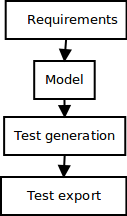
\includegraphics[scale=0.6]{figures/conformiq_process.png}
\caption{MBT process in Conformiq}
\label{fig:conformiq_process}
\end{figure}
	
	\item After the modelling phase, abstract test cases can be generated. The generation starts with transforming the model to an intermediate Lisp model that is used during the symbolic execution, which generates the use cases. The user is able to see coverage statistics and a traceability matrix based on the generated test cases.
	\item Abstract test cases have to be exported, with so called scripting backend, which creates concrete test cases for the SUT.
\end{enumerate}

% section conformiq (end)

\section{GOTCHA}
\label{sec:gotcha}

GOTCHA \cite{gotcha} is a framework that consists of two main components. The first one generates test cases from FSM models, while the others transforms abstract test cases into concrete test cases written in Java and then executes them on the SUT.

The model is described with GDL (GOTCHA Definition Language) that contains states, state variables, actions, expected results and guards. Abstract test cases are generated into XML format. Concrete test cases are executed on the SUT using an adapter that can be written with the help of some helper class. The concrete method mapping is made by an XML file, which maps to specific SUT methods.

% section gotcha (end)

\section{ParTeG}
\label{sec:parteg}

Partition Test Generator \cite{parteg}\cite{partegweb} is an open source Eclipse plugin that can generate test cases from UML models annotated with OCL guards. It traverses the graph representing the UML state machine and each path corresponds to a test case.

The used test case generation algorithm is the following:

\begin{enumerate}
	\item A selected coverage criterion is transformed into model specific test goals.
	\item Each test goal references a concrete element of the model.
	\item From each of these element, a path to the model's initial state represents a test case given by the corresponding transitions.
	\item Backwards on the path, each guard becomes a constraint on the inputs, which will be the initial input parameters in the end.
\end{enumerate}

% section parteg (end)

\section{Conclusions}
\label{sec:conclusions}

After investigating five widely used MBT tools, we can draw some consequence. From our point of view the most important parts of their features are the used modelling notation and the test case (TC) generation methods, because these are the most crucial parts of the design. I summarised the collected information in the Table~\ref{tab:toolssummary}.

\begin{table}[htb]
\begin{center}
\begin{tabular}{llll}\toprule
	\textbf{Name of the tool} & \textbf{Model} & \textbf{Intermediate model} & \textbf{TC generation method}\\\midrule
	GraphWalker & FSM & graph (GraphML) & SBST, combinatorial, random\\
	PyModel & FSM + Python & graph & SBST, random\\
	Conformiq & QML & Lisp (CQ$\lambda$) & symbolic execution\\
	GOTCHA & EFSM & graph & BFS, DFS\\
	ParTeG & UML + OCL & graph & DFS, symbolic execution\\
\bottomrule
\end{tabular}
\end{center}
\caption{\label{tab:toolssummary} Summary of examined MBT tools}
\end{table}

\begin{itemize}
	\item Creators of these tools either try to use an UML like model or FSM (EFSM). FSM models are low level representations of the SUT, so implementing search-based algorithms and graph traversal algorithms are relatively easy.
	
	When engineers choose to use UML with graph intermediate model, they can not support complex UML state chart elements, such as orthogonal regions, because these features are hard to integrate into a graph representation.
	\item The intermediate model is just always some kind of graph representation, because the test case generation algorithms are the easiest to implement using graph models (search-based test case generation, coverage criteria).
	\item Scaffolding solutions of the tools are incomplete. Fully automatic generation of test adapters, oracles are seldom supported. These features make the testing tool more useful, because they accelerate the testing process.
	\item Regression tests are not supported. When an actual error is found, then the SUT should be tested against the generated test suite and this process should be supported by the testing tool.
	\item Only a few tools have an integrated solution to create models. Handling models correctly is an essential feature of model-based testing tools, because an integrated model editor improves the testing process greatly. Testing is an iterative process, so contextual switching between model editor and testing tool results an overhead.
	\item Input models are not verified. Model-based testing the same as other testing methods can only find discrepancies regarding their source. If the test model is not correct, then the tests will be ineffective. That's why that is also important to verify the input model and to help the testing process.
	\item The tools implement different coverage criteria, but even the most general state and transition coverage are not fully supported by each of the tools. More difficult criteria are avoided, for example transition pair, sneak path, all path and scenario coverage.
	
	Transition pair coverage may be avoided because the few added value compared to a full transition coverage. Another reason can be that depending on the actual model and test case generation algorithm, this criterion can be hard to implement properly.
	
	Sneak path means a path that contains an accepted method, which should not be accepted. By a fully specified model each possible transition is represented, so that sneak path criterion is not applicable.
	
	Usage of scenario coverage results reasonable smaller test suite, then the other test selection criteria, but a transition coverage may replace this criterion.
	\item Script-flow criteria are rarely used techniques. Only a few of them support guards, but even those do not report on their coverage. Simple criteria as model flow criteria are not so effective at finding faults, whereas complex criteria like script flow criteria help find different kind of faults. On the other hand complex criteria are also significantly expensive in terms of theoretical complexity.
	\item Requirement traceability are ignored by just all the available tools. This feature make the tools more useful, but does not effect the ability to find more errors. Tracing requirements is rather used by software validation.
\end{itemize}

% section conclusions (end)

% chapter relatedwork (end)
	%TODO Tervezés
	%----------------------------------------------------------------------------
\chapter{Design}
\label{cha:design}
%----------------------------------------------------------------------------

Generating test cases from a specific model based on two step from the model-based testing process (see fourth step at Chapter~\ref{cha:modelbasedtesting}), namely the modelling and test case formalization (test selection criteria, test case specification) phases. These steps will be discussed one by one, considering the previously defined requirements. 

\section{Modeling language}
\label{sec:modelinglanguage}


\subsection{UML state machine}
\label{sub:umlstatemachine}

As the goal is to generate test cases from state machines, that having an UML state machine like semantics, investigating the UML standard \cite{omguml} can not be missed in this thesis.

UML state machines or UML state charts are improved versions of the mathematical concept of finite state automatons expressed with the OMG's Unified Modeling Language. The idea behind this notation is, that an entity or each of its sub-entities is always in exactly one of a number of possible states and where there are well-defined conditional transitions between these states. UML state charts introduce new features over traditional finite automatons such as hierarchically nested regions, orthogonal regions and actions. There are two kinds of state machine, which can be used to define behaviour of model elements and describe protocol usage.

\begin{figure}[htp]
\centering
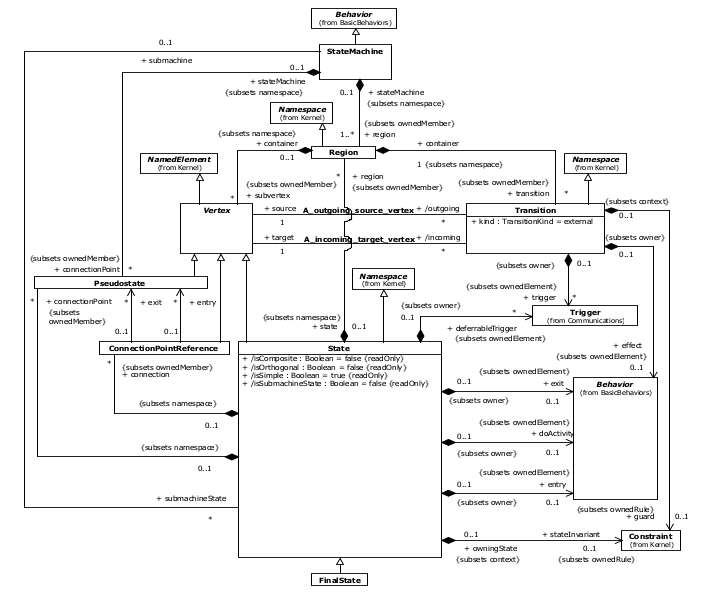
\includegraphics[scale=0.5]{figures/statemachine_metamodel}
\caption{Metamodel of UML state machine}
\label{fig:statemachine_metamodel}
\end{figure}

UML state machines are similar to traditional state machines, the main parts of them are the followings:

\begin{description}
	\item[States] are the phases of the system's history. For example if the history can be separated into two phases, then there are two states. 
	\item[Extended states] represents the complete condition of the system. This interpretation means usually states extended with system variables.
	\item[Transitions] happens when a state switched to another.
	\item[Actions] executed when an event dispatched and the system responds by performing them.
	\item[Events] can be everything, that happens with the system, and causes state change.
	\item[Guards] are boolean expressions described with extended state variables and event parameters. They can affect the system's behaviour by enabling or disabling transitions.
	\item[Hierarchically nested regions] means that if a system is in a substate then it is also in the same time in all the substate's superstates.
	\item[Orthogonal regions] are regions, which are in 'OR' relation.
\end{description}

% subsection umlstatemachine (end)

\subsection{PLC-HSM}
\label{sub:plchsm}

PLC-HSM is a modelling language intended to be a formal,
modular, hierarchical specification for describing PLC programs. It was created as part of a doctoral programme by Dániel Darvas of the Budapest University of Techology and Economics (BUTE) and the European Organization for Nuclear Research (CERN).

\begin{figure}[htp]
\centering
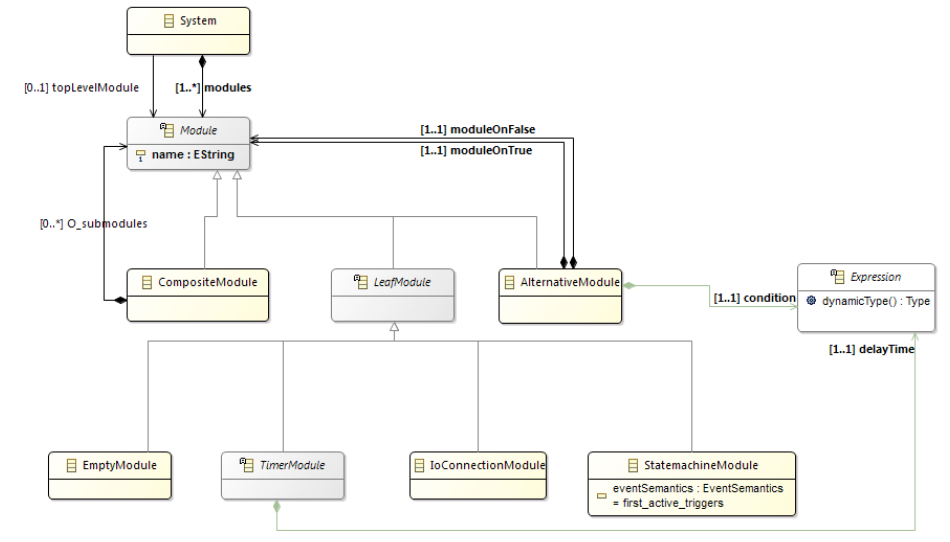
\includegraphics[scale=0.4]{figures/plchsm_modules}
\caption{Module structure of PLC-HSM}
\label{fig:plchsm_modules}
\end{figure}

The specification organized into modules (Figure~\ref{fig:plchsm_modules}), which are either represent a behaviour of concrete module (\texttt{LeafModule}) or they are composite modules containing a set of submodules (\texttt{CompositeModule}). There are four different module type:

\begin{itemize}
	\item \texttt{StatemachineModule} represents an UML-like state machine.
	\item \texttt{IoConnectionModule} defined by connections between input and output variables.
	\item \texttt{TimerModule} describes a PLC timer in the system.
	\item \texttt{EmptyModule} is a module without any state machine or IO connection.
\end{itemize}

From these module types we are interested especially in the state machine notation. As shown on Figure~\ref{fig:plchsm_statemachine} the metamodel is similar to UML state machine's metamodel described in the previous section.

\begin{figure}[htp]
\centering
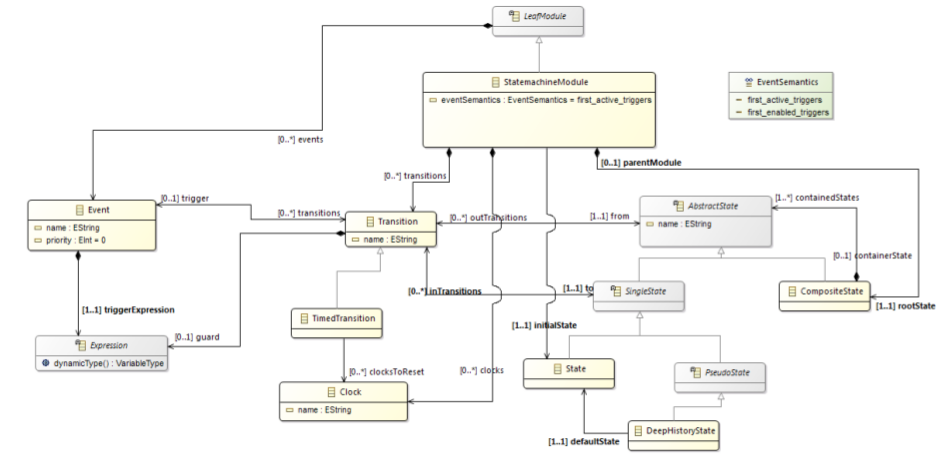
\includegraphics[scale=0.5]{figures/plchsm_statemachine}
\caption{Structure of \texttt{StatemachineModule}}
\label{fig:plchsm_statemachine}
\end{figure}

On the other hand PLC-HSM has some difference from the UML notation:

\begin{itemize}
	\item There is a root state, that recursively contains all of states.
	\item There are pseudo states (\texttt{DeepHistoryState}), which can save a state configuration for its container state.
	\item There are \texttt{TimedTransitions}, which are transitions having time-related conditions.
	\item With \texttt{Clocks} it is possible to define synchronous stopwatches, which can measure the elapsed time since last reset.
	\item Parallel regions are not allowed.
	\item Initial state can not be defined for composite states.
	\item At every moment, exactly one atomic state can be active. 
\end{itemize}

% subsection plchsm (end)

We can see, that PLC-HSM has some advantage over traditional UML modeling language:

\begin{itemize}
	\item UML language has only an informally given semantics.
	\item Tools having UML state machine creating capabilities are not standardised.
	\item PLC-HSM is rather a subset of the UML state machine language, and so it is more simple.
\end{itemize}

% section modelinglanguage (end)

\section{Test generation algorithms}
\label{sec:testgenerationalgorithms}

\subsection{Alloy}
\label{sub:alloy}

Alloy is a formal modeling language to define structures. Alloy can be utilised with a tool, called Alloy Analyzer to automate the verification process. The tool transforms problems into SAT formulas to solve them. The solver was inspired by model checkers, but it is implemented as a solver, performing verification within a bounded scope.

The strength of this tool allows us to define our test generation goals with the Alloy language to generate the test cases. The test cases need to guarantee state-based and transition-based coverages.

% subsection alloy (end)

% section testgenerationalgorithms (end)

% chapter design (end)
	%TODO Implementáció
	%----------------------------------------------------------------------------
\chapter{Implementation}
\label{cha:implementation}
%----------------------------------------------------------------------------

At the end of the design step it is clearly visible, what advantages the investigated technologies and tools have. The implementation of the created testing framework represented following the model based testing process phases as earlier.

\begin{figure}[htp]
\centering
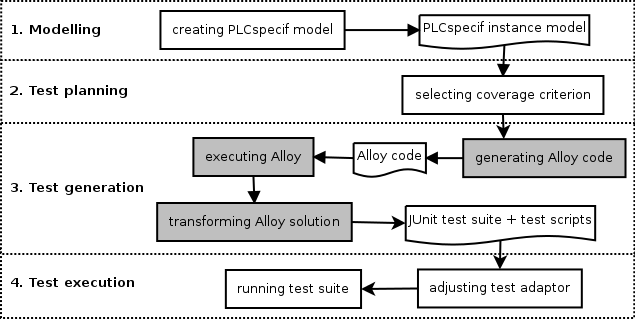
\includegraphics[scale=0.6]{figures/implementation_usage}
\caption{Usage of the test generator framework}
\label{fig:implementation_usage}
\end{figure}

Figure~\ref{fig:implementation_usage} demonstrates the usage of the testing framework. The manual operations are noted with white rectangles, the automatically executed operations are in grey rectangles. Outputs of the operations are represented with document symbols.

The different phases will exemplify the testing of a trivial application, which state machine is showed on Figure~\ref{fig:implementation_trivialsm}. This application has only one method that increases the value of a variable from $0$ to $1$. \texttt{T0} represent the single method the state machine has. Besides that, the state machine has an always satisfiable guard \texttt{G0} , as variable \texttt{output} is initialised to $0$, and an event \texttt{E0} that increases the \texttt{output} variable by $1$. 

\section{Modelling}
\label{sec:implementationmodelling}

First the input model of the testing framework have to be created. This is a PLCspecif instance model created with the default PLCspecif model editor that is generated by the Eclipse Modeling Framework. PLCspecif's generated editor implements all the needed model creation, edition features (UC.1) and model validation as well (UC.2). Concerned components noted on Figure~\ref{fig:designcomponents}, with PLCspecif model, edit framework, model editor and validator.
	
The simplest possible state machine that has all the main UML state machine features showed on Figure~\ref{fig:implementation_model}.
	
\begin{figure}[htp]
\centering
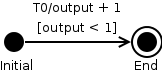
\includegraphics[scale=0.4]{figures/implementation_trivialsm}
\caption{State machine of a trivial SUT}
\label{fig:implementation_trivialsm}
\end{figure}

Constructed models should have some mandatory elements to fully support the test generation process e.g. the JUnit test case generation. The modelled system should have only one state machine module (\texttt{TrivialSM}), where the test model is realised. Each state machine should have a \texttt{VariableDeclaration} named \texttt{output}, one \texttt{CompositeState}, that contains all the \texttt{BasicState}s, from which two has the name \texttt{Initial} and \texttt{End} accordingly.
	
\begin{figure}[htp]
\centering
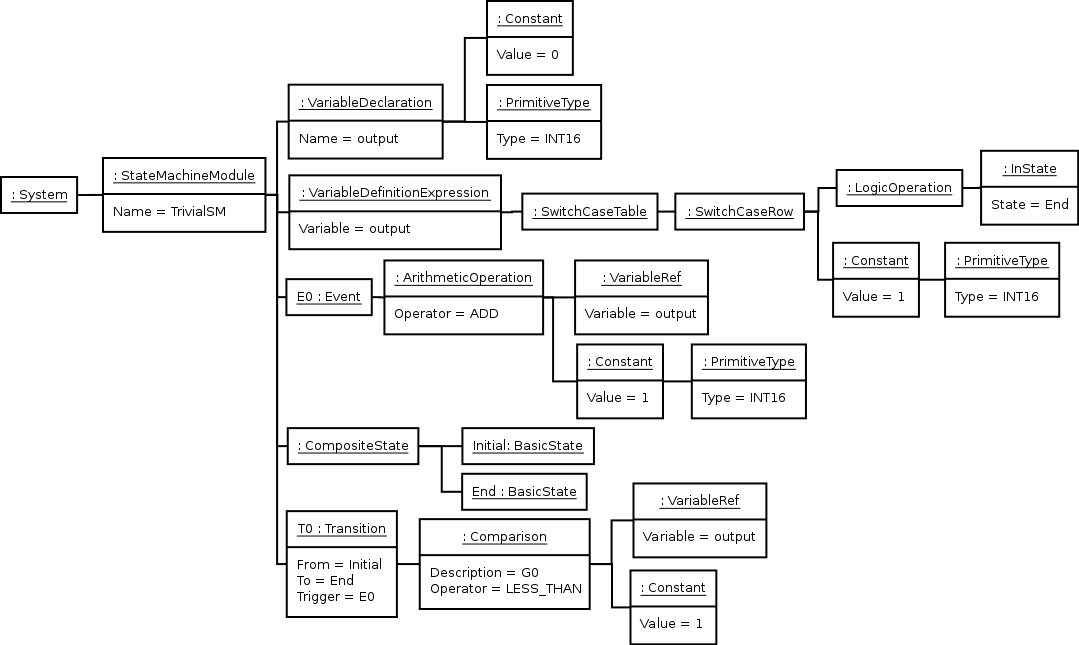
\includegraphics[scale=0.4]{figures/implementation_model}
\caption{Object diagram of a PLCspecif instance model}
\label{fig:implementation_model}
\end{figure}
	
Output assignments is described with a specific \texttt{VariableDefinitionExpression} for \texttt{output} variable. Outputs defined by a switch-case like structure, that has as many \texttt{SwitchCaseRow} as states defined in the state machine. Each row has a condition definition (usually a \texttt{LogicOperation} with a check, that verifies whether the state machine is in a particular state e.g. \texttt{End} state), and a value definition (here represented by a simple \texttt{Constant}). In other words the output of the state machine will be $1$ in the state \texttt{End}.

Transitions can have guard (for example \texttt{G0}) defined on them using \texttt{Comparison} objects. Here \texttt{output} is checked, whether it is less than $1$. Transitions may have attached \texttt{Event}s. For example \texttt{E0} increases the variable \texttt{output} by $1$.

% section modellingimplementation (end)

\section{Test planning}
\label{sec:testplanningimplementation}

At this phase the user can select a test selection criterion (namely full state or transition coverage), which will be used by the test generation. This component is implemented in a separate Eclipse plugin (Test suite generator UI on Figure~\ref{fig:designcomponents}), as the selection is made on the user interface and it is always a good practice to decouple the UI from the business logic.
	
\begin{figure}[htp]
\centering
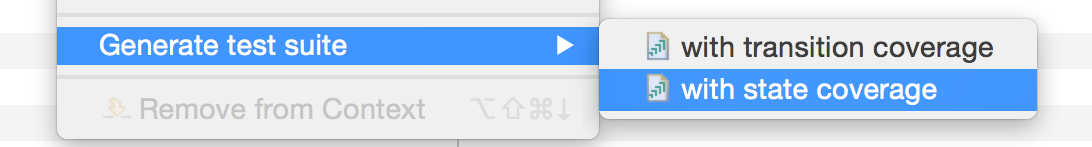
\includegraphics[scale=0.4]{figures/implementation_screenshot}
\caption{Screenshot of the test selection criterion}
\label{fig:implementation_screenshot}
\end{figure}
	
Eclipse SDK exports an extension point \texttt{org.eclipse.ui.popupMenus}, where the context menu of the application can be extended with new actions. So this Eclipse plugin contains two extension, which use this interface to add two new popup menu items.
	
% section testplanningimplementation (end)
	
\section{Test generation}
\label{sec:testgenerationimplementation}
	
When the user selects a test selection criterion on the user interface the test suite generation process will be started automatically. At first the test generation problem will be transformed into Alloy code, that can produce the test cases. The required informations can be extracted from the previously created PLCspecif model, and so the desired Alloy code can be generated automatically. This generation was solved with the model to text transforming capabilities of Acceleo and implemented in a separate Eclipse plugin (Test suite generator on Figure~\ref{fig:designcomponents}).
	
The generated Alloy code has two main parts, the first one consists of statically generated code parts, the other includes highly dynamical, customised structures.
	
Listing~\ref{lst:alloystatic} shows the static parts of the generated Alloy code. Basic structural metamodel of state machines are implemented with signatures (line number  \ref{lst:static1start}-\ref{lst:static1end}). \texttt{System} represents the internal state of the state machine by its state variables. \texttt{State}, \texttt{Transition} objects refer to the traditional EFSM elements. Each state knows its internal state through the \texttt{System} object, and each transitions connects two states.
	
From lines \ref{lst:static2start}-\ref{lst:static2end} metamodel of basic testing object are described. \texttt{Coverage} can refer to a state or transition coverage and so it can be transformed to a test suite. \texttt{Path} is set of method calls within the software, generally more path serve as a \texttt{Coverage}. \texttt{Step} is a method call in the context of software behaviour, but it also connects testing objects to state machine objects.
	
The helper function \texttt{steps} returns a relation containing all steps from a given path. From line number \ref{lst:static3start}-\ref{lst:static3end} are the basic rules of the system. Most of the rules describe the semantics of either the behaviour of state machines or the testing objects. Testing specific model consistency is also verified.

The predicate \texttt{inheritSystem}, is similar to a helper function, but it can only return boolean values if its constraints are satisfiable. This predicate is used to pass along the internal state of the system between the different states.
	
\begin{lstlisting}[label={lst:alloystatic}, caption=Static parts of the generated Alloy code,breaklines=true]
abstract sig System {}(*@\label{lst:static1start}@*)
abstract sig State {system: one System}
abstract sig Transition {from, to: one State}(*@\label{lst:static1end}@*)

sig Coverage { paths: some Path }(*@\label{lst:static2start}@*)
sig Path { firstStep: one Step }
sig Step {
  from, to: one State,
  via: one Transition,
  nextStep: lone Step
} {
  via.from = from
  via.to = to
}(*@\label{lst:static2end}@*)
fun steps (p:Path): set Step { p.firstStep.*nextStep }
fact {(*@\label{lst:static3start}@*)
  // test generation properties
  all p:Path | one c:Coverage | p in c.paths // all path belongs to a coverage
  all s:Step | one p:Path | s in p.firstStep.*nextStep // all steps belongs to a path

  // model consistency
  all p:Path | p.firstStep.from = Initial // all path starts with an Initial state
  all p:Path | one s:Step | s in steps[p] && s.to = End // all path ends with End state
	
  // state machine properties
  all curr:Step, next:curr.nextStep | next.from = curr.to // all steps are continuous
  all sys:System | some s:State | sys = s.system // all system belongs to a state
}(*@\label{lst:static3end}@*)
pred inheritSystem(s1, s2: System) { s1 = s2 }
\end{lstlisting}

Listing~\ref{lst:alloydynamic} shows the dynamic parts of the generated Alloy code. These parts of the Alloy code are generated using the previously created PLCspecif instance model (Figure~\ref{fig:implementation_model}).

Instance models of the \texttt{State} signatures (\texttt{Initial}, \texttt{End}) are instantiated using inheritance. Concrete transitions (\texttt{T0}) are inherited from the \texttt{Transition} object as well. Transitions connected to the initial state have to initialise the internal state variables of the state machine using the dynamically generated \texttt{initSystem} predicate. Guards (\texttt{G0}) and events (\texttt{E0}) connect to these transition objects too.

\begin{lstlisting}[label={lst:alloydynamic}, caption=Dynamic parts of the generated Alloy code,breaklines=true]
one sig Initial, End extends State {}
some sig S extends System {
  output: Int
}
lone sig T0 extends Transition {}{
  from = Initial
  to = End
  initSystem[from.system]
  E0[from.system, to.system]
  G0[from.system]
}
pred E0(s1, s2: System) {
  s2.output = add[s1.output, 1]	
}
pred G0(s: System) {
  s.output < 1
}
pred initSystem(s:System) {
  s.output = 0
}
\end{lstlisting}

Finally Listing~\ref{lst:alloycriteria} show the test criteria formalisation by Alloy predicates. A possible test suite guarantees state coverage if all state present in the union of start and end states of all step in the coverage. Transition coverage is defined in a similar way: a test suite guarantees transition coverage if all transition can be mapped to a step in the coverage.

These criteria are applicable using Alloy's \texttt{run} statements. The constraint solving is executed in a bounded scope, that's why the scope of the search for examples need to be calculated dynamically.

\begin{lstlisting}[label={lst:alloycriteria}, caption=Formalising criteria with Alloy,breaklines=true]
pred state_coverage() {
  all s:State | some p:Path | s in steps[p].from + steps[p].to
}
pred transition_coverage() {
  all t:Transition | some p:Path | t in steps[p].via
}
run state_coverage for 10 but exactly 1 Coverage, 2 System
\end{lstlisting}

The above described generated Alloy code are executed automatically using the Alloy Analyzer API. Operational parameters and other options were fine tuned to get the best possible performance from the integrated SAT solvers. The process of this research will be detailed in Chapter~\ref{cha:measurements}.

When the model is satisfiable and a possible coverage is generated, the solution is parsed into an internal model representation. This internal model is closely related to the testing level and is rather the metamodel of a JUnit test suite.

Similarly to PLCspecif, this internal notation uses a customised Ecore metamodel to describe its behaviour. Instead of starting with a default Ecore model editor, this metamodel is constructed using annotated Java interfaces. Based on them an Ecore model and a generator model is constructed, which will generate the remaining code.

The Alloy solution parser is based on the \textit{Builder} pattern and uses model \textit{Factory} classes from EMF.Edit to create the internal model. After building the test suite model, Acceleo transforms automatically this model to text representation including a complete JUnit test suite (see on Listing~\ref{lst:testsuite}) with pure POJO helper classes.

\begin{lstlisting}[label={lst:testsuite}, caption=Generated JUnit test suite,breaklines=true]
package trivialsm;

import org.junit.Before;
import org.junit.Test;

import junit.framework.TestCase;

public class TrivialSMTest extends TestCase {
	protected TrivialSM trivialsm = null;
	protected TrivialSMTestAdapter adapter = null;
	   
	@Before 
	public void setUp() {
		trivialsm = new TrivialSM();
		adapter = new TrivialSMTestAdapter(trivialsm);
	}
	
	@Test
	public void testPath1() {
		assertEquals(1, adapter.T0());
	}
}
\end{lstlisting}

% section testgenerationimplementation (end)

\section{Test execution}
\label{sec:testexecutionimplementation}

Output of the test generation process consists of three scaffolded helper classes (showed on Figure~\ref{fig:implementation_testhelpers}). They are all generated automatically, derived from the generated test cases and the test model.
	
\begin{description}
	\item[Test suite] is generated as a standard JUnit test fixture (see \texttt{TrivialSMTest} in Listing~\ref{lst:testsuite}). The different test paths are separated into annotated test methods (e.g. \texttt{testPath1}), and a \texttt{setUp} method can be used to initialise the test adapter. Test oracles are generated dynamically in the form of single assertions and inserted into the test methods.
	
	The generated test suite can contain more test paths, which include usually more test cases. A single path starts from the initial state of the SUT and ends in the end state. Set of the paths offer full state or transition coverage within the SUT.
	
	When the user re-generates a test suite for the SUT it can differ from the previously generated test suite, although the generated test suite will have the same structural properties as earlier. This anomaly is, because the execution of the included SAT solver is undetermined.
	\item[Test adapter] scaffolded as a simple POJO class (\texttt{TrivialSMTestAdapter}). This class maps the model transitions to concrete method calls, and also initialisation of the SUT can be done in the adapter's constructor. Method calls wired automatically to concrete SUT's method, using a simple heuristic. If the mapping is not trivial, the adapter's code may not be perfect and needs some adjustment. Here the SUT, named \texttt{TrivialSM} is quite simple, and the adapter does not need any further modification.
	
\begin{figure}[htp]
\centering
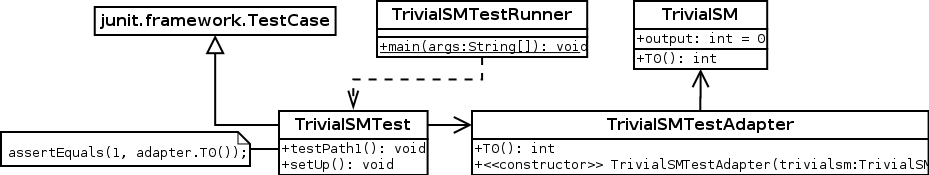
\includegraphics[scale=0.45]{figures/implementation_testhelpers}
\caption{Class diagram of the scaffolded test helpers}
\label{fig:implementation_testhelpers}
\end{figure}

	\item[Test script] is a simple JUnit test runner (\texttt{TrivialSMTestRunner}) that reports the result of the testing. It works like the default JUnit test runner, so it reports out the result of the complete test suite execution (Listing~\ref{lst:successfultestsuite}).

\begin{lstlisting}[label={lst:successfultestsuite}, caption=Successful test suite execution output,breaklines=true]
Finished in 0.005 seconds
1 examples, 0 failures, 0 ignored
\end{lstlisting}
	
	The test reporter tells the difference between the expected and the actual test outcome, moreover if some discrepancy is found it shows the stack trace of the actual exception (Listing~\ref{lst:failedtestsuite}).

\begin{lstlisting}[label={lst:failedtestsuite}, caption=Failed test suite execution output,breaklines=true]
Finished in 0.007 seconds
1 examples, 1 failures, 0 ignored
Failed examples:
testPath1(trivialsm.TrivialSMTest)
junit.framework.AssertionFailedError: expected:<1> but was:<2>
...
\end{lstlisting}
	
\end{description}
	
% section testexecutionimplementation (end)

% chapter implementation (end)
	%TODO Skálázás és mérések
	%----------------------------------------------------------------------------
\chapter{Scaling and measurements}
\label{cha:measurements}
%----------------------------------------------------------------------------

After each implementation iteration I measured the performance of the created framework, and continued the development using the results of these measurements. As we previously saw the heart of the framework is the SAT solver, which is also the most time consuming part of the system. So the best way to improve the speed of the execution is to improve the underlying Alloy program.

I created a testing tool to measure the execution of the different Alloy programs. This testing tool can be configured to compare the execution of different Alloy programs, with different execution strategy. The execution strategy can mean different SAT solvers, and other solver configurations as well.

Execution of each testing configuration was measured 10 times and the results in the following section always refer to average metrics. The tests has been running on the configuration that can be seen in Table~\ref{tab:hardwarespecification}.

\begin{table}[htb]
\begin{center}
\begin{tabular}{|l|}
\hline
	\textbf{Hardware specification}\\\hline
	\textbf{CPU}: 2.7GHz dual-core Intel Core i5 processor with 3MB shared L3 cache\\
	\textbf{RAM}: 8GB 1866MHz LPDDR3 RAM\\
	\textbf{Storage}: 128GB PCIe-based flash storage\\
\hline
\end{tabular}
\end{center}
\caption{\label{tab:hardwarespecification} Measurement architecture}
\end{table}

\section{Alloy settings}
\label{sec:alloysettings}

During the first measurement I experimented with the available solvers supported by Alloy and their solver specific configurations. Alloy Analyzer supports huge variety of SAT solvers and they have a decent number of tuning possibility.

I was able to integrate seven different SAT solvers into the system, namely CryptoMiniSat, Glucose, MiniSat, MiniSat with core extraction, Sat4j, Lingeling and its parallel version Plingeling. The another dimension of the measurement was the SAT solver configuration. Settings of two configuration was not obvious, that's why I chose to measure these parameters.

The first investigated option was Skolem-depth that controls the maximum depth of alternating universal and existential quantifier when generating a Skolem function. Minimum value is 0, which means it will only generate Skolem constants, and will not generate Skolem functions, maximum value is 4, where Skolem functions are generated in depth of 4.

\begin{figure}[htp]
\centering
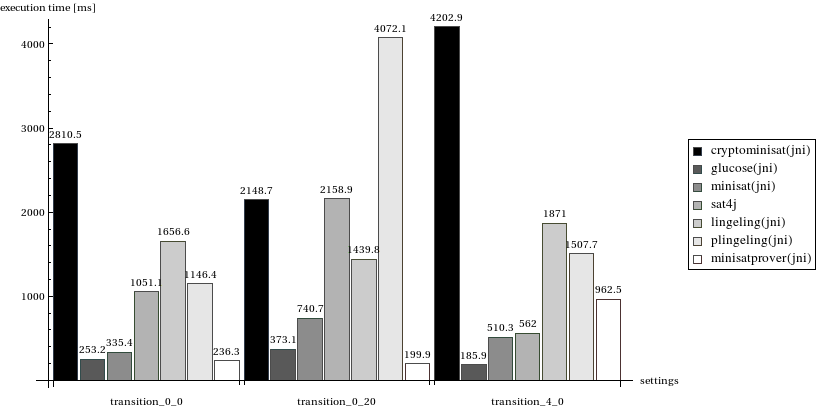
\includegraphics[scale=0.55]{figures/measurements_alloy_settings}
\caption{Adjusting Alloy settings}
\label{fig:measurements_alloy_settings}
\end{figure}

Second option to inspect was symmetry breaking. The official documentation suggests that  if a formula is unsatisfiable, then in general, the higher this value, the faster the solver will finish. On the other hand, if the formula is satisfiable, then the value should be set to a lower value. Minimum of symmetry breaking is 0, maximum is 20.

Figure~\ref{fig:measurements_alloy_settings} shows the results of the measurement. On the x-axis are the solver configurations in the form: \mbox{<\textit{test selection criterion}>\_<\textit{Skolem-depth}>\_<\textit{symmetry breaking}>}. On y-axis is the execution time, and the different colours represent different SAT solver implementations.

The result was similar with state and transition coverage criteria as well, therefore here only the transition coverage version is demonstrated. Measurement with Skolem-depth of 4 and symmetry breaking of 20 is not presented, because this configuration could not satisfy the given problem in acceptable period of time.

The fastest solver became the award winning Glucose SAT solver. Only the MiniSat solvers could approach the performance of Glucose, the other solvers seemed to be significantly slower. That's why Glucose became the default solver of the testing framework.

Symmetry breaking with a value of 0 was also a clear choice, since the documentation suggest, that the programs solves satisfiable problem with a lower value more easily. 

Changing the Skolem-depth did not impact the speed very much, only a small amount of difference could be measured. Glucose was faster with an option 0, which was also the default value, so I did not change that.

% section alloysettings (end)

\section{Optimisations}
\label{sec:optimalisations}

After the first measurements the performance of the test generation seemed to be adequate to work with, but as I increased the complexity of the problems to solve, so increased the execution time of the test generation. 

\begin{figure}[htp]
\centering
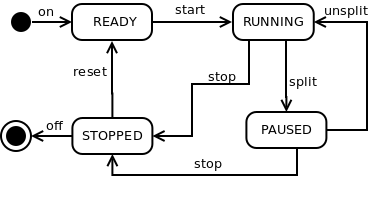
\includegraphics[scale=0.5]{figures/measurements_stopwatch}
\caption{Stopwatch FSM for testing}
\label{fig:measurements_stopwatch}
\end{figure}

As an input for the testing tool I designed an example FSM that represents a simplified stopwatch behaviour (Figure~\ref{fig:measurements_stopwatch}). This FSM is ideal for testing purposes, because on the test suite of this stopwatch full state and transition coverage can be achieved and therefore both of the implemented algorithms can be tested.

In the first development iteration, the test generation algorithm could not generate test cases for this FSM within a tolerable time. This was a huge problem, as it could jeopardise the success of using constraint solving methods for test generation. After examining the test generation process and the results with Alloy Analyzer, I identified the main issues.

The first problem was that the model was overconstrained and that's why the SAT solver generated to much variables, while parsing the given constraints. The other problem was that, the solver generated different objects in a scenario for the same purpose, that's why state space increased exponentially.

\begin{figure}[htp]
\centering
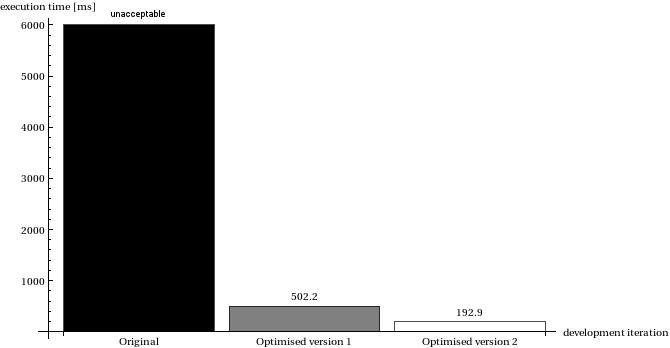
\includegraphics[scale=0.55]{figures/measurements_optimalizations}
\caption{Optimisations results}
\label{fig:measurements_optimalizations}
\end{figure}

Solution for these problems are the same: the Alloy model needs to be simplified. This has been done in two steps,  Figure~\ref{fig:measurements_optimalizations} shows the effects of the optimisations. After deleting the unneeded constraints from the model, each SAT solver could solve the stopwatch problem. The execution time at this time displayed with the label "Original" on Figure~\ref{fig:measurements_optimalizations}. Later I modified the model to reuse the previously generated model objects to reduce the state explosion.

The speed of the execution increased radically during these optimisations. In the first step, the increase can not be calculated, as the speed was unacceptable in the first version. Considering the speed of the chosen SAT solver, Glucose, the execution became twice as faster, than preciously between the second and the third version of the test generation algorithm.

% section optimalizations (end)

\section{Scalability}
\label{sec:scalability}

In the first measurement I investigated the scalability of the created testing framework. I assumed that the test generation algorithm does not scale equally regarding the number of states or transitions generated during the test case generation. That's why I measured the performance considering these two options.

First applicable PLCspecif models have to be generated in different sizes, that are input models of the framework. Then the test generation process can be started using these models where the execution speed is measurable.

Creating a random PLCspecif model, that can represent a SUT, where different test selection criteria can be satisfied is not an easy task, as it involves complex graph theory algorithms to generate such a graph representation. Main parts of the process are the following:

\begin{enumerate}
	\item At first graph model of the SUT have to be generated. Process of the graph generation is demonstrated in Algorithm~1.
	
\begin{algorithm}
\label{alg:sutmodelgeneration}
\SetAlgoLined
\KwData{$n, t$ such that $t$ is the type of the generation scope for a $G(V,E)$ graph,\\
and $n=$
\begin{cases}
|V|, $ if $ t = $ state$\\
|E|, $ if $ t = $ transition$
\end{cases}
}
\KwResult{$G(V,E)$ graph representation of the SUT}
$s \leftarrow 0$\;
\While{$s \neq n$}{
$in\_degree\_sequence \leftarrow [0] + \mathrm{random\ sequence} + [1]$\;
$out\_degree\_sequence \leftarrow [1] + \mathrm{random\ sequence} + [0]$\;
\While{$|in| \neq |out|$}{
$out\_degree\_sequence \leftarrow [1] + \mathrm{random\ sequence} + [0]$\;
}
$G(V,E) \leftarrow$ random directed pseudograph, using the degree sequences\;
\If{$\exists e \in E: e=(v,v): v \in V$} {
$E\leftarrow E \setminus e$\;
}
$s =$\begin{cases}
|V|, $ if $ t = $ state$\\
|E|, $ if $ t = $ transition$
\end{cases}
}
\caption{Generating SUT models based on the size of states or transitions}
\end{algorithm}

	The graph will be generated randomly using previously defined in/out-degree sequences. FSM models always have an initial and an end state, which have an in-degree 0 and 1, and out-degree 1 and 0 consequently. The generated model has to support one of our test selection criteria to be able to execute later with our testing tool, so I chose to implement state coverage support on the generated models, as it is more simple than the transition coverage. FSMs having a full state coverage need to have all state with incoming and outgoing transitions, thus all state will be reachable. These rules are formalised in lines 3-7.
	
	Generated graph should not have self-loops, as triggering transitions always initiates a state change (line number 9-11).
	
	The resulted graphs was exported into GraphML format.
	
	\item  Exported graphs are transformed into PLCspecif model notation using generated factories offered by the EMF platform. First skeleton model of a SUT is created by code, which is filled later with the states and transitions coming from the parsed GraphML graphs.
	
\end{enumerate}

Figure~\ref{fig:measurements_scalability} shows the results of the scalability measurements. As I assumed previously the framework scales differently regarding the number of states or transitions, that the SUT has.

\begin{figure}[htp]
\centering
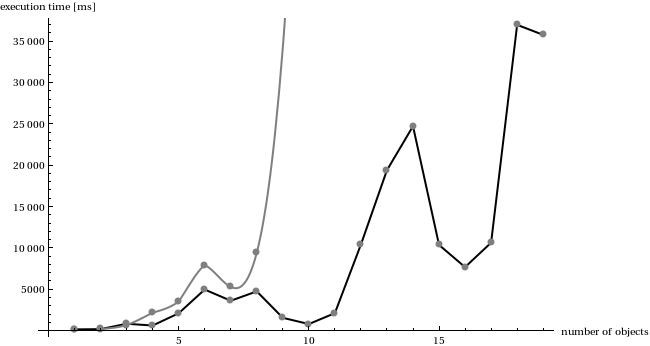
\includegraphics[scale=0.5]{figures/measurements_scalability}
\caption{Scalability results regarding the number of states or transitions}
\label{fig:measurements_scalability}
\end{figure}

The created model based testing framework performs well, while generating test suites for medium sized models. Practically that means SUT with 5-10 states and 15-20 transitions are solvable by this tool. In this range the execution speed varies under 35 seconds, which is an acceptable speed.

Used input models were randomly generated test models, that's why the complexity of solving these problems does not perfectly follows the increase of the concerned testing objects. Besides that we can see a trend line, that the execution speed increases linear or polynomial at first, but later it will grow exponentially regarding the number of states or transitions.

Important to note that the number of states in the SUT model, affects the execution speed more, than the number of transitions, as possible states of the \texttt{System} (set of internal variables) are bound to the \texttt{State} objects in the Alloy model. So as the number of states increases, so does the possible value assignments for internal variables increases.

% section scalability (end)

% chapter measurements (end)
	%TODO Értékelés és továbbfejlesztési lehetőségek
	%----------------------------------------------------------------------------
\chapter{Summary and further development}
\label{cha:summary}
%----------------------------------------------------------------------------

In this chapter first I position and categorise the created model-based testing software in a way presented in Chapter~\ref{cha:modelbasedtesting} and in Chapter~\ref{cha:relatedwork}. Utting, Pretschner and Legeard \cite{taxonomy} defined a taxonomy for categorising tools based on their test model and the used test generation algorithms, while Shafique and Labiche \cite{toolsreview} identified the key features of MBT tools and classified them according to these criteria. Showing what the finished tool is capable of can be presented easier using these classifications.

Summarising the work is followed by the possibilities of further development and improvements. These statements are either proven with the results of the measurements or defined by the need for new features that the available tools lack of.

Finally I will end this thesis with the final results and personal experiences.

\section{Positioning of the thesis}
\label{sec:positioning}

The taxonomy and the tools review protocol describe the most important aspects of a model-based testing tool. We can use the same methods to evaluate the developed testing tool and see how it differs from other tools.

Table~\ref{tab:toolevaluation} shows the results of this evaluation. On one hand the created tool is very similar to the available testing tools. Most of them use some FSM or UML like modelling notation. This is not so surprising, because one of the main goal of this thesis was to generate test suites for state-based models, which implicated to use untimed, deterministic, discrete transition based models. Preferring structural model coverage criteria, moreover concentrating on model-flow criteria is a similarity as well. Nevertheless implementing such a criteria is the easiest, that's why support most of the available testing tools them, when using state based models.

\begin{table}[htb]
\begin{center}
\begin{tabular}{p{4cm}p{3.5cm}p{6.5cm}}
\toprule
	\textbf{Property} & \textbf{Value} & \textbf{Notes} \\\midrule
	Subject of testing & \textit{SUT} & The test model represent the SUT, not its environment. \\
	Test model separation & \textit{Separated} & Different model is used for testing and development.\\
	Model characteristics & \textit{Deterministic}, \textit{untimed}, \textit{discrete} & Possibility to support timed transitions. \\
	Model paradigm & \textit{Transition based} & PLCspecif state machine notation.\\
	Test selection criteria & \textit{Structural model coverage} & Full state and transition coverage are supported.\\
	Test generation technology & \textit{Constraint solving} & Generating test cases using Alloy. \\
	Test execution & \textit{Offline} & - \\\midrule
	Model-flow criteria & \multicolumn{2}{p{10.5cm}}{\textit{Transition} and \textit{state coverage} are supported; transition-pair, all-path coverage are not. Sneak-path and scenario coverage are not applicable, because the model is always considered complete and modifying the search for test cases is impossible, because the test generation technology.} \\
	Script-flow criteria & \multicolumn{2}{p{10.5cm}}{\textit{Interface}, \textit{statement}, \textit{decision} coverage are supported implicitly, others are not applicable, because the test generation technology.} \\
	Data and requirements criteria & \multicolumn{2}{p{10.5cm}}{Not supported.} \\
	Test scaffolding criteria & \multicolumn{2}{p{10.5cm}}{\textit{Adapter creation}, \textit{oracle automation} are supported. \textit{Stub creation are not supported.}} \\
	Related activities criteria & \multicolumn{2}{p{10.5cm}}{\textit{Model creation}, \textit{model verification}, \textit{test case debugging}, \textit{test case debugging}, \textit{regression testing} are fully supported. Requirements traceability is not supported.} \\
\bottomrule
\end{tabular}
\end{center}
\caption{\label{tab:toolevaluation} Applied techniques and supported features of the created tool}
\end{table}

On the other hand this new testing tool is unique. Constraint solving as test generation technology is a rare choice. Though it is a useful method by test generation as we saw earlier. Other strengths of this tool are the full support of test scaffolding and related activities criteria. From the reviewed tools only a few can support all these features in one integrated framework. 

% setion positioning (end)

\section{Possibilities for further development}
\label{sec:furtherdevelopment}

\begin{description}
	\item[Better scalability] After some development iteration the created framework is able to solve real world problems, but as the number of state increases in the SUT model, the tool's execution speed enlarges exponentially.
	
	On the one hand it can be problem if the goal is to generate test suite for a complex SUT, but on the other using complex state machine features in a big SUT model is certainly not recommended. When developers use a state machine like model, usually the used state machine are not so complicated.
	
	Either way the execution speed can be improved. The improvement can be achieved with more option:
	
	\begin{itemize}
		\item The most time consuming part of the system is the Alloy test generation, which can be improved by generating less runtime objects, while solving a SAT formula. Alloy model has to be simplified to do this.
		\item Input model can be simplified before transforming to Alloy too. Solving easier parts of the models separately can also reduce the state space, therefore the constraint solving part will be faster. The easy parts of the system can be solved with other test generation methods e.g. with graph algorithms.
	\end{itemize}
	\item[Support more PLCspecif features] Currently the testing tool supports most of the elements from the PLCspecif feature set. However some basic UML like element are not supported, for example composite states and pseudo states as deep history states.
	
	Guards and events also can not be defined arbitrary. These elements may benefit from the usage of the whole expression model. Expressions have an extensive metamodel and currently only the binary operations are supported. Supporting the other operations may improve the usability of the testing framework.
	\item[Requirements traceability] Requirements traceability can be defined as documenting the life of a requirement. In the field of software testing it also means the reporting of the requirements coverage.
	
	Possible scenarios to support this feature can be the following:
	
	\begin{itemize}
		\item Creating a traceability matrix may help to check if the current requirements are being met or can help in the creation of a requirements specification. When a requirements is accomplished it should be noted on test models. Regarding these information traceability matrices can be filled during the test case generation.
		\item Third party requirement management tool integration can also help in a similar way as traceability matrices.
	\end{itemize}
\end{description}

% setion furtherdevelopment (end)

\section{Conclusions}
\label{sec:conclusions}

Regarding the previously defined requirements, I successfully created a model-based testing framework based on state machine models.

\begin{itemize}
	\item I presented the main goals of model-based testing and the general testing process.
	\item I investigated the related work that use state machine models for generating tests.
	\item I chose a state machine modelling notation and designed a framework that is able to generate complete test suites with previously defined test selection criteria.
	\item I implemented the testing framework and described its internal behaviour.
	\item Finally I evaluated the finished solution and sketched some possible future work.
\end{itemize}

After the testing and measurements phases I have concluded that the resulted testing framework is able to complete the tasks and to satisfy the requirements that were defined at the start of the work. The software can maybe fill a gap, because it was designed to offer solutions to problems, that the other tools can not solve.

During the development of this software I continuously learned new technologies and algorithms. Finally I can say that it was a wonderful experience to design and develop a complete and useful solution for such a complex and hard problem.

% setion conclusions (end)

% chapter summary (end)


% List of Figures, Tables
%~~~~~~~~~~~~~~~~~~~~~~~~~~~~~~~~~~~~~~~~~~~~~~~~~~~~~~~~~~~~~~~~~~~~~~~~~~~~~~~~~~~~~~
	\listoffigures\addcontentsline{toc}{chapter}{\abrakjegyzeke}
	\pagenumbering{roman}
	\setcounter{page}{\value{romanPage}}
	\listoftables\addcontentsline{toc}{chapter}{\tablazatokjegyzeke}


% Bibliography
%~~~~~~~~~~~~~~~~~~~~~~~~~~~~~~~~~~~~~~~~~~~~~~~~~~~~~~~~~~~~~~~~~~~~~~~~~~~~~~~~~~~~~~

	\addcontentsline{toc}{chapter}{\irodalomjegyzek}
	\nocite{*}
	\bibliographystyle{plain}
	\bibliography{/Users/municsovics/GoogleDrive/school/MSc/3. félév/Onlab1/msc-thesis/doc/dipterv2/bib/unicsovicsmilangyorgy_jzk4.bib}


% Appendix
%~~~~~~~~~~~~~~~~~~~~~~~~~~~~~~~~~~~~~~~~~~~~~~~~~~~~~~~~~~~~~~~~~~~~~~~~~~~~~~~~~~~~~~
	%----------------------------------------------------------------------------
\appendix
%----------------------------------------------------------------------------
\chapter*{\fuggelek}\addcontentsline{toc}{chapter}{\fuggelek}
\setcounter{chapter}{6}  % a fofejezet-szamlalo az angol ABC 6. betuje (F) lesz
\setcounter{equation}{0} % a fofejezet-szamlalo az angol ABC 6. betuje (F) lesz
\numberwithin{equation}{section}
\numberwithin{figure}{section}
\numberwithin{lstlisting}{section}
%\numberwithin{tabular}{section}


\label{page:last}
\end{document}
